\subsection{Hardware design Switch board}
I det følgende afsnit beskrives designet af hardwaren til switch boardet. Switch boardet er udviklet således at fjernbetjeningen kan overtage styringen fra main controlleren.

På figur \ref{fig:switchboard_design} ses det overordnede design til switch boardet. 
De respektive PWM signaler skal ind i en 2-input AND gate hvor hver PWM signal har en AND gate. Den anden indgang bruges af et kontrol pin som styres af main controlleren. Denne pin sættes enten høj eller lav, afhængigt af hvilken enhed der skal styre dronen. 
De AND gates der har med samme PWM styring at gøre (fx. Throttle) sendes til en OR gate som sender PWM signalet videre til flight control boardet. 

\begin{figure}[H]
	\centering
	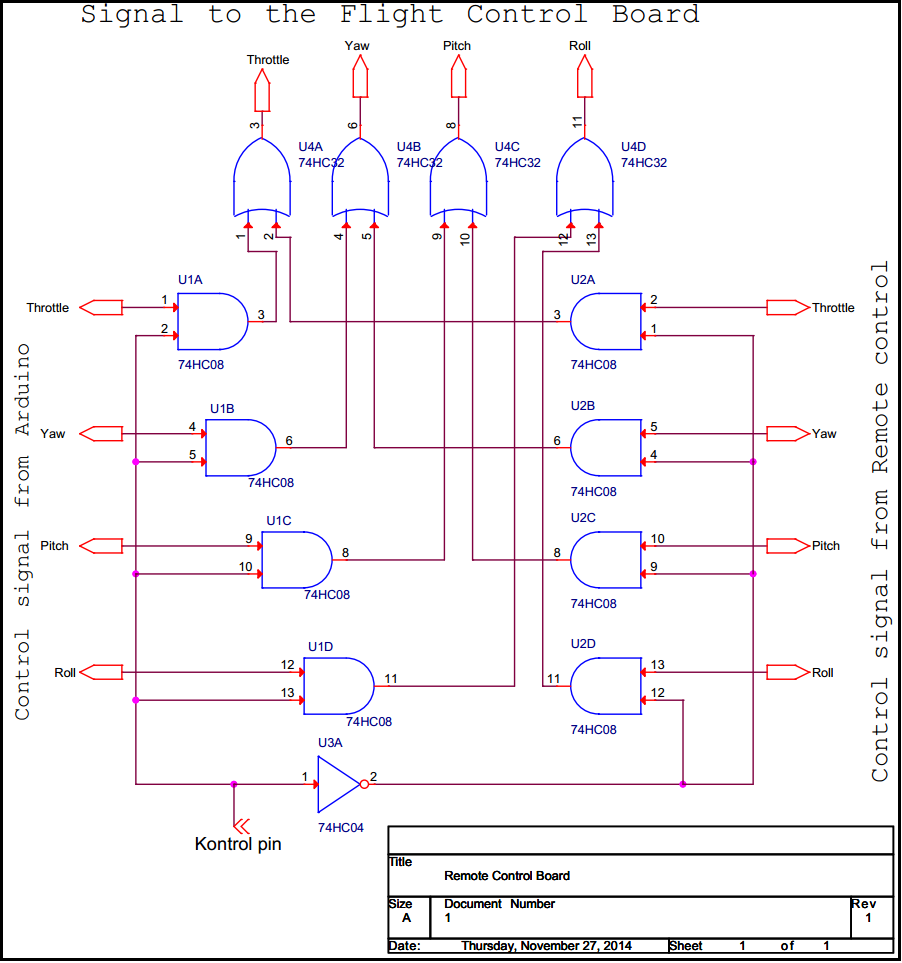
\includegraphics[width=1\textwidth]{Billeder/hardware/switch_board_diagram.png}
	\caption{Switch board design}
	\label{fig:switchboard_design}
\end{figure}
